\documentclass[11pt,compress,t,notes=noshow, xcolor=table]{beamer}
\input{../../style/preamble_new}
\input{../../latex-math/basic-math.tex}
\input{../../latex-math/basic-ml.tex}

\title{Deep Learning for NLP}

\definecolor{texblue}{rgb}{0, 0, 1}
\def\myblue#1{\textcolor{texblue}{#1}}
\long\def\devour#1{}

\definecolor{texblue}{rgb}{0, 0, 1}
\def\myblue#1{\textcolor{texblue}{#1}}


\begin{document}

%\devour{

\titlemeta{
Training LLMs
}{
Memory and compute requirements
}{
figure/float.png
}{
\item Learn about different contributions to compute requirements
\item Learn how model size components influence memory requirements
}


% ------------------------------------------------------------------------------

\begin{vbframe}{From Transformer Architecture to Training Cost}

\vfill

You already know how a Transformer is built.

Now we want to turn its architecture into concrete numbers:

\begin{itemize}
    \item \textbf{How many parameters does it have?}
    \begin{itemize}
        \item How do $d_{\text{model}}$, number of layers, and other
        architectural choices determine model size?
    \end{itemize}

    \item \textbf{How much compute does training require?}
    \begin{itemize}
        \item How do model size and number of training tokens determine
        the number of operations?
    \end{itemize}

    \item \textbf{How much GPU memory does training require?}
    \begin{itemize}
        \item Parameters are only one part: we also need to store
        gradients, optimizer states, and activations.
    \end{itemize}
\end{itemize}

\centering
\textbf{Architecture $\;\longrightarrow\;$ parameters
$\;\longrightarrow\;$ compute and memory}

\vfill

\end{vbframe}

% ------------------------------------------------------------------------------

\begin{vbframe}{Where Are the Parameters in a Transformer Block?}

\vfill

A decoder Transformer block mainly contains parameters in
\textbf{self-attention} and the \textbf{feed-forward network (MLP)}.

\textbf{Self-attention:}

\begin{itemize}
    \item Query, key, and value projections:
    \[
        W_Q,\; W_K,\; W_V
        \qquad
        d_{\text{model}} \times
        (n_{\text{heads}} d_{\text{head}})
    \]
    \item Output projection:
    \[
        W_O
        \qquad
        (n_{\text{heads}} d_{\text{head}})
        \times d_{\text{model}}
    \]
\end{itemize}

\textbf{Feed-forward network (MLP):}

\begin{itemize}
    \item Two weight matrices, typically with hidden dimension
    $4d_{\text{model}}$:
    \[
        d_{\text{model}} \times 4d_{\text{model}}
        \qquad\text{and}\qquad
        4d_{\text{model}} \times d_{\text{model}}
    \]
\end{itemize}

In the standard Transformer,
\[
    n_{\text{heads}} d_{\text{head}} = d_{\text{model}}.
\]

\vfill

\end{vbframe}

% ------------------------------------------------------------------------------

% ------------------------------------------------------------------------------

\begin{vbframe}{Parameter Count of One Transformer Block}

Using $n_{\text{heads}} d_{\text{head}} = d_{\text{model}}$, self-attention ($W_Q, W_K, W_V, W_O$) contributes

\[
P_{\text{attn}}
=
4 d_{\text{model}}^2
\]

The MLP contributes

\[
P_{\text{MLP}}
=
2 \cdot d_{\text{model}} \cdot 4d_{\text{model}}
=
8d_{\text{model}}^2.
\]

Hence,

\[
\boxed{
P_{\text{block}}
=
12d_{\text{model}}^2
}
\]

and for $n_{\text{layers}}$,

\[
\boxed{
P_{\text{blocks}}
=
12n_{\text{layers}}d_{\text{model}}^2
}
\]


\end{vbframe}


% ------------------------------------------------------------------------------

\begin{vbframe}{Does the Approximation Work?}

\textbf{GPT-3 Small} ($n_{\text{layers}}=12,\ d_{\text{model}}=768$): \citebutton{Brown et al., 2020: GPT-3}
{https://arxiv.org/abs/2005.14165}
\[
P_{\text{blocks}}
\approx
12 \cdot 12 \cdot 768^2
\approx
85\text{M}.
\]
Actual model size: \textbf{125M parameters}.

\textbf{GPT-3 Medium} ($n_{\text{layers}}=24,\ d_{\text{model}}=1024$):
\[
P_{\text{blocks}}
\approx
12 \cdot 24 \cdot 1024^2
\approx
302\text{M}.
\]
Actual model size: \textbf{350M parameters}.

\textbf{What is missing? Mainly the token embeddings.}

For vocabulary size $|\mathcal V|$,
\[
P_{\text{embed}} = |\mathcal V|\,d_{\text{model}}.
\]

GPT-3 has $|\mathcal V|\approx 50{,}000$, hence approximately
\[
P_{\text{embed}}
\approx
39\text{M}\ \text{(Small)},\qquad
51\text{M}\ \text{(Medium)}.
\]

Other parameters (e.g., LayerNorms and biases) are comparatively small.

\end{vbframe}

% ------------------------------------------------------------------------------
% ------------------------------------------------------------------------------

\begin{vbframe}{Training Compute: Forward Pass}

Let $P$ be the number of parameters and $D$ the number of training tokens.

For one token, each parameter participates in roughly one
multiply-add operation.

A multiply-add costs approximately $2$ FLOPs:

\[
a \cdot b + c
\]

Therefore, over $D$ training tokens,

\[
\boxed{
C_{\text{forward}} \approx 2PD
}
\]

Hence, forward-pass compute grows linearly with

\begin{itemize}
    \item the number of model parameters $P$,
    \item the number of training tokens $D$.
\end{itemize}

\end{vbframe}

% ------------------------------------------------------------------------------

\begin{vbframe}{Training Compute: Backward Pass}

In the forward pass, a layer computes

\[
Y = XW.
\]

During backpropagation, it must compute

\begin{itemize}
    \item gradients for the weights $W$,
    \item gradients for the layer input $X$
          (to continue backpropagation).
\end{itemize}

Both require matrix multiplications of similar size to the forward pass.

Thus, backward costs roughly twice as much as forward:

\[
C_{\text{backward}} \approx 4PD.
\]

Together,

\[
\boxed{
C \approx 2PD + 4PD = 6PD
}
\]

\end{vbframe}


% ------------------------------------------------------------------------------
\begin{vbframe}{From FLOPs to Training Time}

Training requires $C \approx 6PD$ floating-point operations.\\

If the hardware achieves throughput $\tau$ FLOP/s, then 
\[
\boxed{
T \approx \frac{C}{\tau}
=
\frac{6PD}{\tau}
}
\] \citebutton{Source: Quentin et al., 2023}{https://blog.eleuther.ai/transformer-math/}


\textbf{Example:} 7B parameters trained on 1T tokens:

\[
C
\approx
6 \cdot 7\cdot10^9 \cdot 10^{12}
=
4.2\cdot10^{22}\text{ FLOPs}.
\]

Training can be distributed across multiple GPUs. Ideally,

\[
\tau
\approx
n_{\text{GPU}}
\cdot
\tau_{\text{GPU}}.
\]

In practice, communication and synchronization prevent ideal linear scaling.

\end{vbframe}


% ------------------------------------------------------------------------------

\begin{vbframe}{A Fixed Compute Budget Leaves a Choice}

Training compute is approximately

\[
C \approx 6PD,
\]

where

\begin{itemize}
    \item $P$ = number of model parameters,
    \item $D$ = number of training tokens.
\end{itemize}

For a fixed compute budget $C$,

\[
PD \approx \text{constant}.
\]

So we can choose between, for example,

\begin{itemize}
    \item a \textbf{larger model} trained on fewer tokens,
    \item a \textbf{smaller model} trained on more tokens.
\end{itemize}

\begin{center}
\textbf{Which choice gives the best model?}
\end{center}

This question (and similar tradeoffs) is addressed by \textbf{scaling laws}.

\end{vbframe}

% ------------------------------------------------------------------------------

\begin{vbframe}{What Occupies GPU Memory?}

\textbf{How big will the model be in bytes? Will it fit on my GPU?}

Memory is approximately

\[
\text{number of stored values}
\times
\text{bytes per value}.
\]

For \textbf{inference}, we mainly store

\begin{itemize}
    \item model parameters,
    \item activations.
\end{itemize}

Training additionally requires

\begin{itemize}
    \item gradients,
    \item optimizer states.
\end{itemize}

Thus, $\boxed{
M_{\text{train}}
=
M_{\text{params}}
+
M_{\text{grad}}
+
M_{\text{opt}}
+
M_{\text{activ}}
}$
\vskip3mm
$M_{\text{params}}, M_{\text{grad}}$, and $M_{\text{opt}}$ scale with the number of parameters. Activation memory $M_{\text{activ}}$ also depends on sequence length and batch size.
\end{vbframe}

% ------------------------------------------------------------------------------

% ------------------------------------------------------------------------------

\begin{vbframe}{Floating-Point Precision}

Floating-point numbers use bits for

\begin{itemize}
    \item the sign,
    \item the exponent,
    \item the significand.
\end{itemize}

Two common 16-bit formats are:

\[
\begin{array}{c|ccc}
 & \text{sign} & \text{exponent} & \text{significand} \\
\hline
\text{FP16} & 1 & 5 & 10 \\
\text{BF16} & 1 & 8 & 7
\end{array}
\]

BF16 uses more bits for the exponent and fewer for the significand:

\begin{itemize}
    \item larger dynamic range,
    \item lower numerical precision.
\end{itemize}

Both require $\boxed{2\text{ bytes/value}}$.\\
For comparison, FP32 requires $4$ bytes/value.

\end{vbframe}

% ------------------------------------------------------------------------------

\def\nocaphack{https://mlabonne.github.io/blog/posts/Introduction_to_Weight_Quantization.html}


\begin{vbframe}{FP32/FP16 (\citebutton{(Maxime Labonne)}{\nocaphack})}

\hspace{-0.8cm} 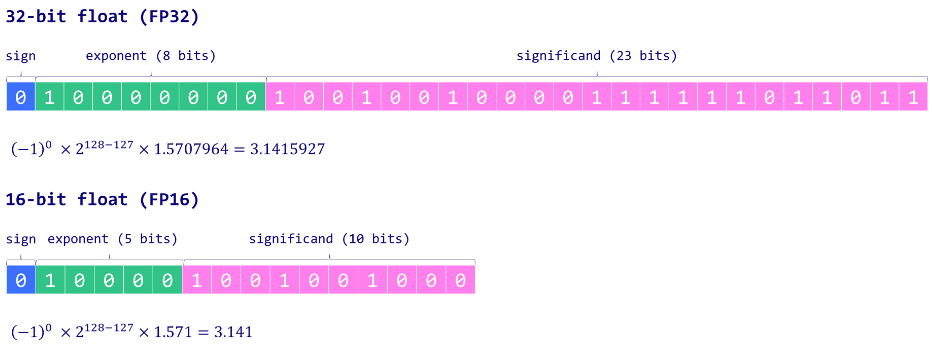
\includegraphics[width = 1.05\textwidth]{./figure/float.png} 



You can represent every float like this:
$(-1)^{\textcolor[RGB]{59,112,254}{S}}\cdot 2^{\textcolor[RGB]{49,195,135}{e}-bias} \cdot 1.\textcolor[RGB]{255,128,237}{m}$\\
(bias = 15 for FP16, 127 for BF16/FP32)

\vskip3mm

Modern accelerators also support FP8 and even FP4
for selected training operations; mixed precision remains an active
area of research.

\end{vbframe}

% ------------------------------------------------------------------------------

\begin{vbframe}{Training Memory per Parameter}

Assume BF16 parameters and gradients, and AdamW.

For each parameter, training stores:

\[
\begin{array}{l|c}
\text{Quantity} & \text{Memory} \\
\hline
\text{BF16 parameter} & 2\text{ bytes} \\
\text{BF16 gradient} & 2\text{ bytes} \\
\text{FP32 Adam momentum} & 4\text{ bytes} \\
\text{FP32 Adam variance} & 4\text{ bytes}
\end{array}
\]

For a model with $P$ parameters:

\[
\boxed{
M_{\text{params+grad+opt}}
\approx
12P\text{ bytes}
}
\]

\textbf{Example:} for a 7B-parameter model,

\[
12 \cdot 7\cdot10^9
=
84\text{ GB}.
\]

This does \textbf{not} yet include activation memory.

\end{vbframe}

% ------------------------------------------------------------------------------

\begin{vbframe}{Will My Model Fit on a GPU?}

Consider a 7B-parameter model.

\[
\text{BF16 parameters: } 2 \cdot 7\cdot10^9 = 14\text{ GB}
\]

\[
\text{Training state: } 12 \cdot 7\cdot10^9 = 84\text{ GB}
\]

Activations add further memory and depend strongly on batch size,
sequence length, and architecture.

\citebutton{Lv et al., ACL 2024}
{https://aclanthology.org/2024.acl-long.445/}
report about \textbf{31\% activation memory} for one LLaMA-7B setup.

Activation memory can often be traded for extra \emph{re-}computation (\emph{activation checkpointing}):

\[
\boxed{\text{less memory} \;\Longleftrightarrow\; \text{more compute}}
\]

\end{vbframe}


\endlecture
\end{document}
